\documentclass{beamer}
\usepackage{../../shared/styles/custom}






\title{Maths for ML II}
\date{\today}
\author{Nipun Batra}
\institute{IIT Gandhinagar}
\begin{document}
  \maketitle



\begin{frame}{Contour Plot}

	$z = f(x,y) = x^{2} + y^{2}$\\

	\begin{figure}[htp]
		\centering
		\begin{notebookbox}{https://nipunbatra.github.io/ml-teaching/notebooks/contour.html}
		  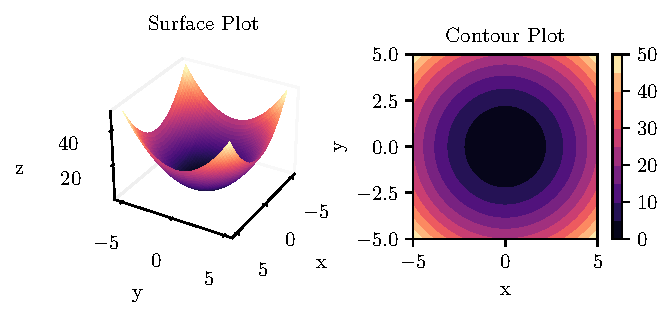
\includegraphics[width=\linewidth]{../assets/mathematical-ml/figures/contour-x_squared_plus_y_squared.pdf}
		\end{notebookbox}
	  \end{figure}

Then plot $f(x,y)=K$ for varying K.

\end{frame}


\begin{frame}{Contour Plot}

$z = f(x,y) = x^{2}$\\

\begin{figure}[htp]
	\centering
	\begin{notebookbox}{https://nipunbatra.github.io/ml-teaching/notebooks/contour.html}
	  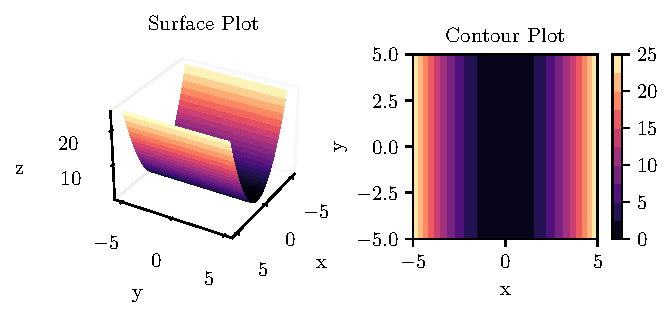
\includegraphics[width=\linewidth]{../assets/mathematical-ml/figures/contour-x_squared.pdf}
	\end{notebookbox}
  \end{figure}

\end{frame}

\begin{frame}{Contour Plot}

$z = f(x,y) = |x|+|y|$\\

\begin{figure}[htp]
	\centering
	\begin{notebookbox}{https://nipunbatra.github.io/ml-teaching/notebooks/contour.html}
	  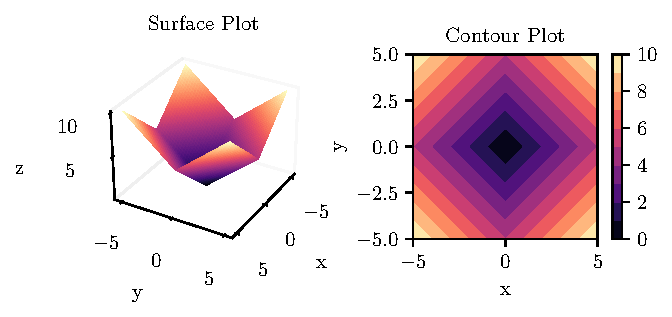
\includegraphics[width=\linewidth]{../assets/mathematical-ml/figures/contour-mod_x_plus_mod_y.pdf}
	\end{notebookbox}
  \end{figure}

\end{frame}

\begin{frame}{Contour Plot}

$z = f(x,y) = (x^2)*y$\\

\begin{figure}[htp]
	\centering
	\begin{notebookbox}{https://nipunbatra.github.io/ml-teaching/notebooks/contour.html}
	  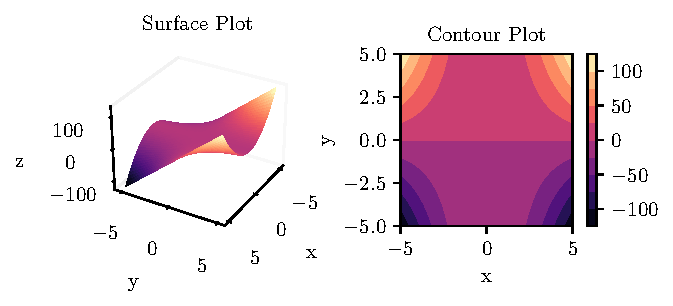
\includegraphics[width=\linewidth]{../assets/mathematical-ml/figures/contour-x_square_times_y.pdf}
	\end{notebookbox}
  \end{figure}


\end{frame}


\begin{frame}{Contour Plot}

$z = f(x,y) = xy$\\

\begin{figure}[htp]
	\centering
	\begin{notebookbox}{https://nipunbatra.github.io/ml-teaching/notebooks/contour.html}
	  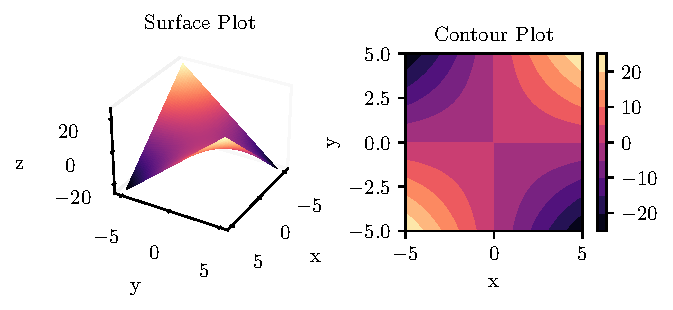
\includegraphics[width=\linewidth]{../assets/mathematical-ml/figures/contour-x_times_y.pdf}
	\end{notebookbox}
  \end{figure}

\end{frame}









\begin{frame}{Contours plots and gradients}
    
    
    Gradient denotes the steepest change.\\
    All points on the contour have the same $f(x,y)$\\
    
    
\end{frame}

\begin{frame}{Contour Plot And Gradients}

$z = f(x,y) = x^{2} + y^{2}$\\

\begin{figure}[htp]
	\centering
	\begin{notebookbox}{https://nipunbatra.github.io/ml-teaching/notebooks/contour.html}
	  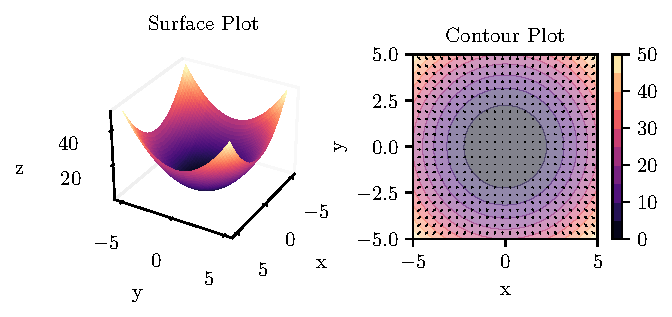
\includegraphics[width=\linewidth]{../assets/mathematical-ml/figures/contour-x_squared_plus_y_squared-with-gradient.pdf}
	\end{notebookbox}
  \end{figure}


\end{frame}








\begin{frame}{Contour Plots and Gradients}
    
    Gradient denotes the direction of steepest descent.\\
    All points on the contour have the same f(x,y).\\
    Gradient denotes the direction in which there is a maximum increase in f(x,y)\\

    
    
\end{frame}





\end{document}
